\documentclass[10pt,usenames,dvipsnames]{beamer}
\usetheme{Madrid}
\usepackage[utf8]{inputenc}
\usepackage{xspace}
\usepackage{graphicx,graphics} 
\usepackage{color}
\usepackage{xcolor}
\usepackage{amsmath}
\usepackage{amsfonts}
\usepackage{amssymb}
\usepackage{amsthm}
\usepackage{algorithm}
\usepackage{algorithmic}
\usepackage{longtable}
\usepackage{complexity}
\usepackage{tkz-graph}
\usepackage{float}
\usepackage{multicol}
\usepackage{setspace}
\usepackage[backend=bibtex,style=verbose]{biblatex}
\addbibresource{src.bib}
\graphicspath{{fig/}}

\title{Apports du couplage et de la monotonie dans la simulation temps parallèle}

\author{Jean-Michel Fourneau, Maël~Guiraud, Yann Strozecki}


\institute[DAVID-UVSQ] 
{
  DAVID, Universit\'e de Versailles Saint Quentin
}

\subject{Theoretical Computer Science}

\begin{document}

\begin{frame}

  \titlepage
  \centering
  
\includegraphics [width=15mm]{logod.png} \hspace{1cm}
\includegraphics [width=20mm]{logo.png} \\
\end{frame}


\begin{frame}{Introduction Simulation temps parallèle}
  \centering
   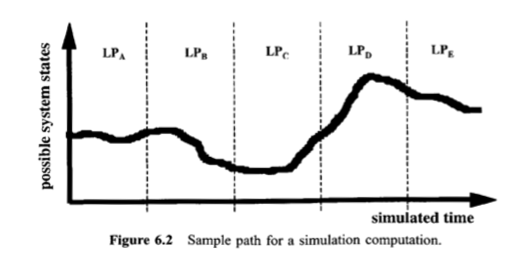
\includegraphics [width=\textwidth]{tmps.png} 
   
    \cite{fujimoto2000parallel}

\end{frame}




\begin{frame}{Introduction Simulation temps parallèle}
  \centering
   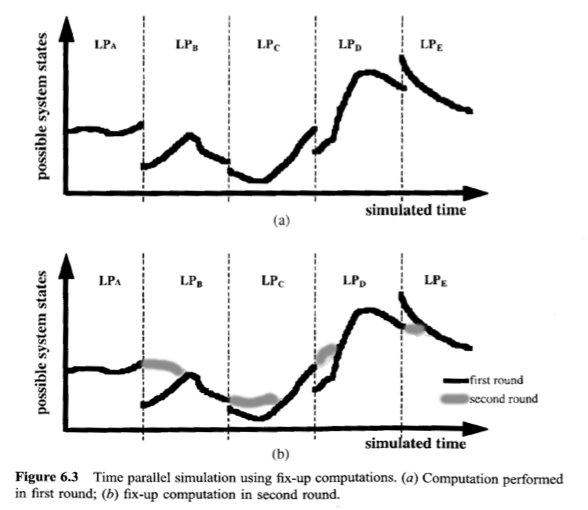
\includegraphics [width=0.7\textwidth]{fuji.png} 
   
\end{frame}

\begin{frame}{Hypothèse sur les états}
  \centering
Pour améliorer la simulation temps parallèle , on fait les suppositions suivantes:
  \begin{itemize}
  \item Un ordre partiel rapidement calculable sur l'ensemble des états
  \item Une monotonie de la dynamique de la chaine de markov
  \item Un état minimum et un état maximum
  \end{itemize}
   
\end{frame}

\begin{frame}{Algorithme à deux bornes (Speculative sandwich)}
  \centering
  Idée de l'algorithme : 
  
  Utiliser une \textcolor{ForestGreen}{borne inférieure} et une \textcolor{red}{borne supérieure} jusqu'au \textcolor{blue}{couplage} des deux trajectoires.
  
	   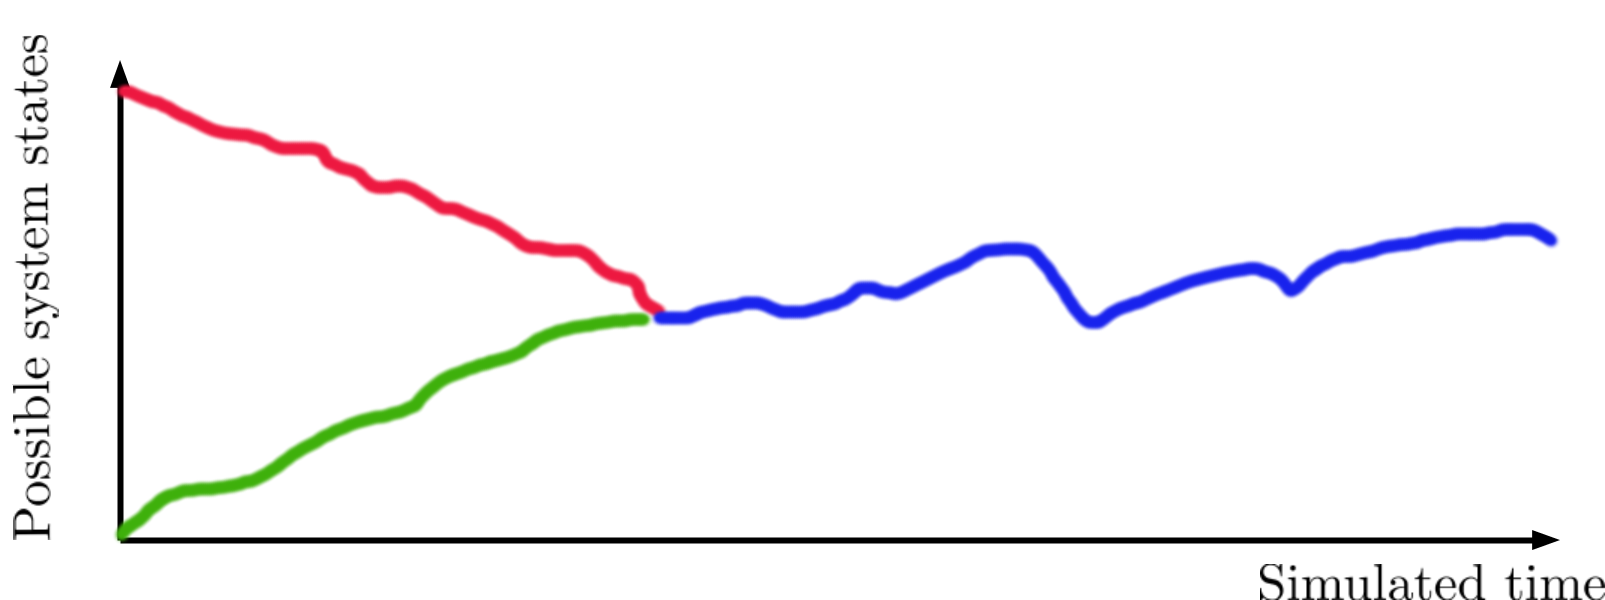
\includegraphics [width=\textwidth]{coupling} 
\end{frame}


\begin{frame}{Algorithme à deux bornes (Speculative sandwich)}
  \centering
	   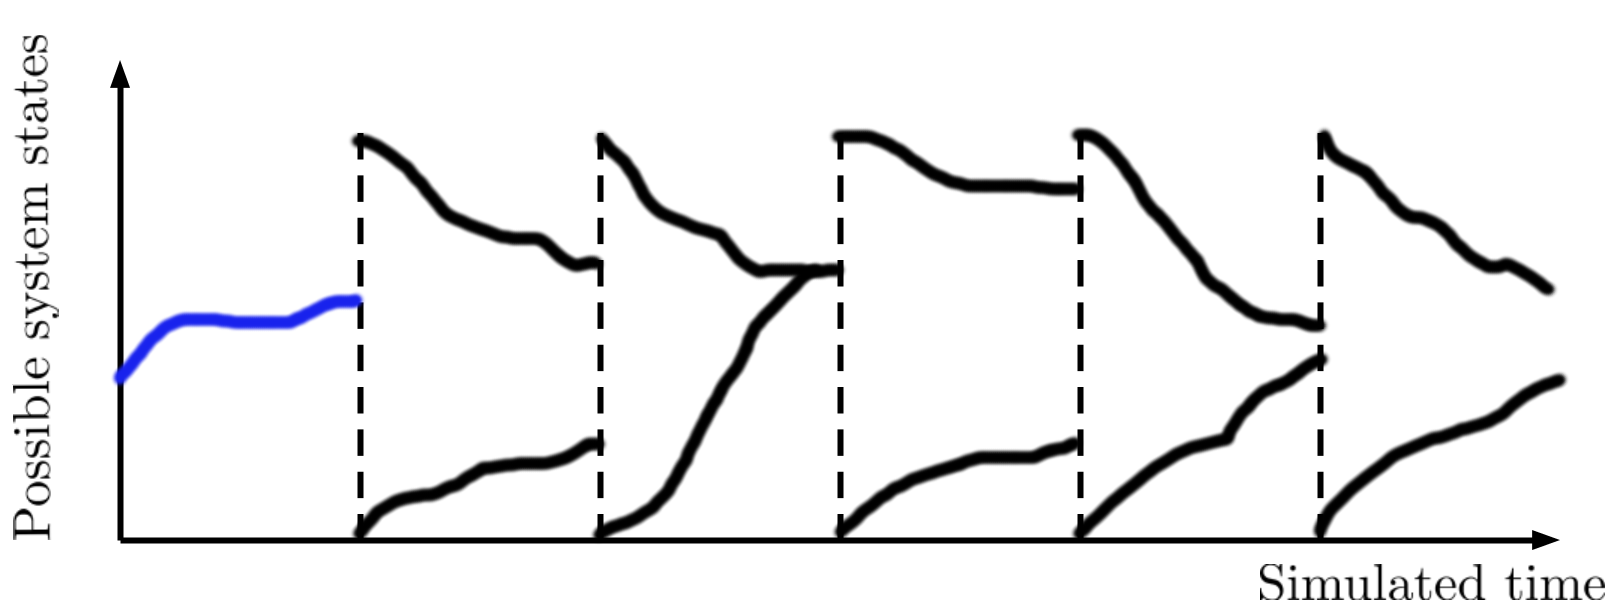
\includegraphics [width=\textwidth]{step0} 
	   
	   Step 1
\end{frame}

\begin{frame}{Algorithme à deux bornes (Speculative sandwich)}
  \centering
	   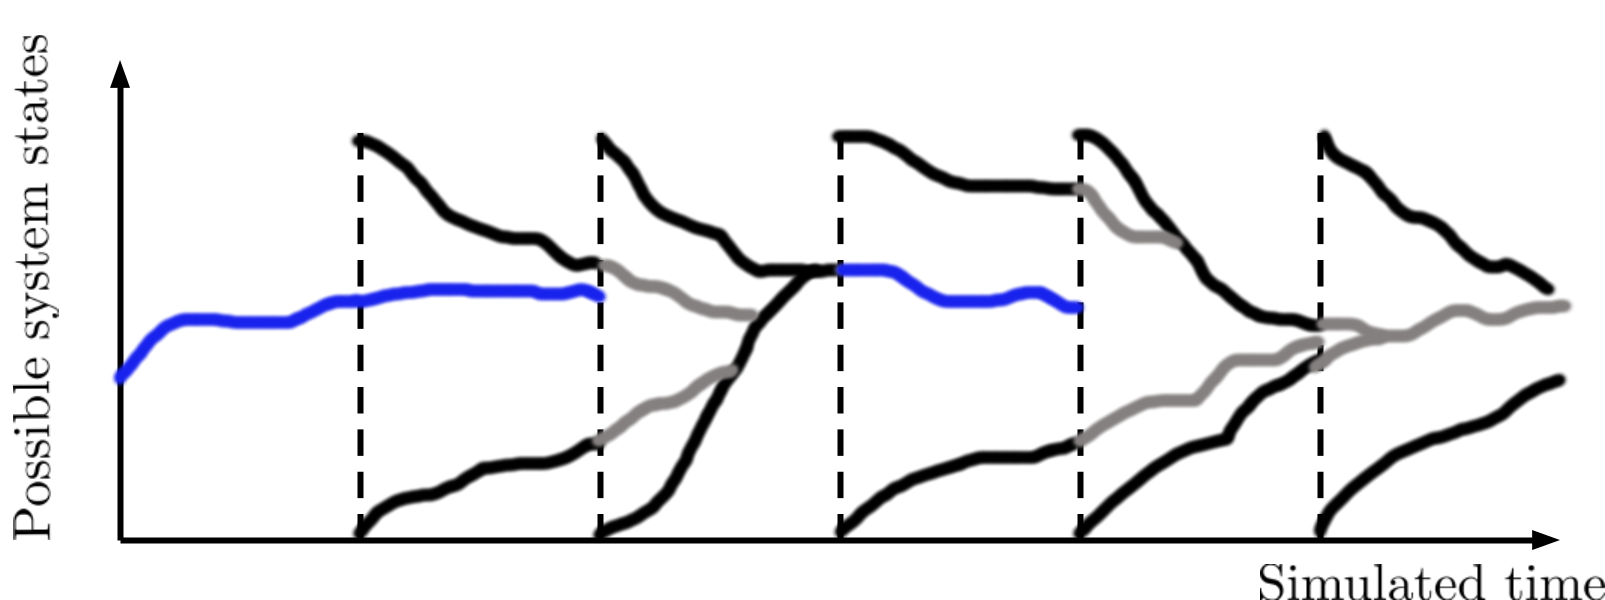
\includegraphics [width=\textwidth]{step1} 
	   
	   Step 2
\end{frame}

\begin{frame}{Algorithme à deux bornes (Speculative sandwich)}
  \centering
	   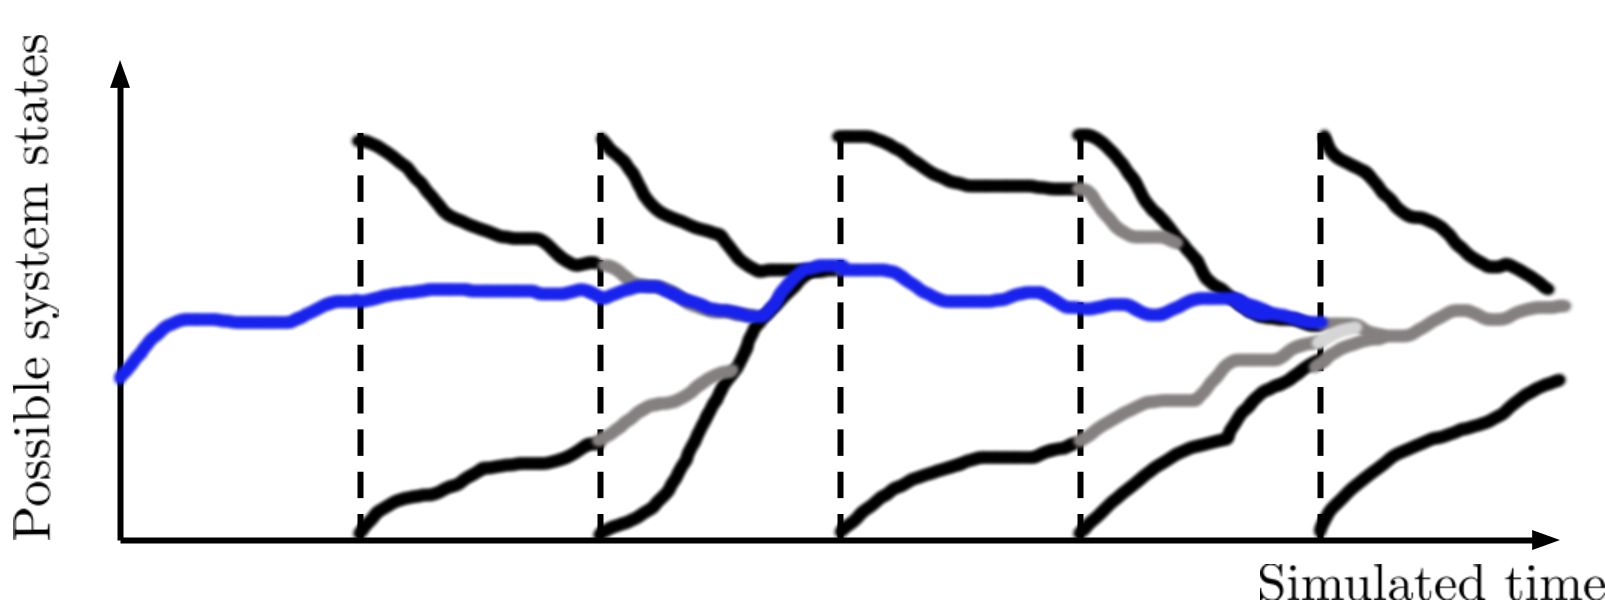
\includegraphics [width=\textwidth]{step2} 
	   
	   Step 3
\end{frame}
\begin{frame}{Algorithme à deux bornes (Speculative sandwich)}
  \centering
	   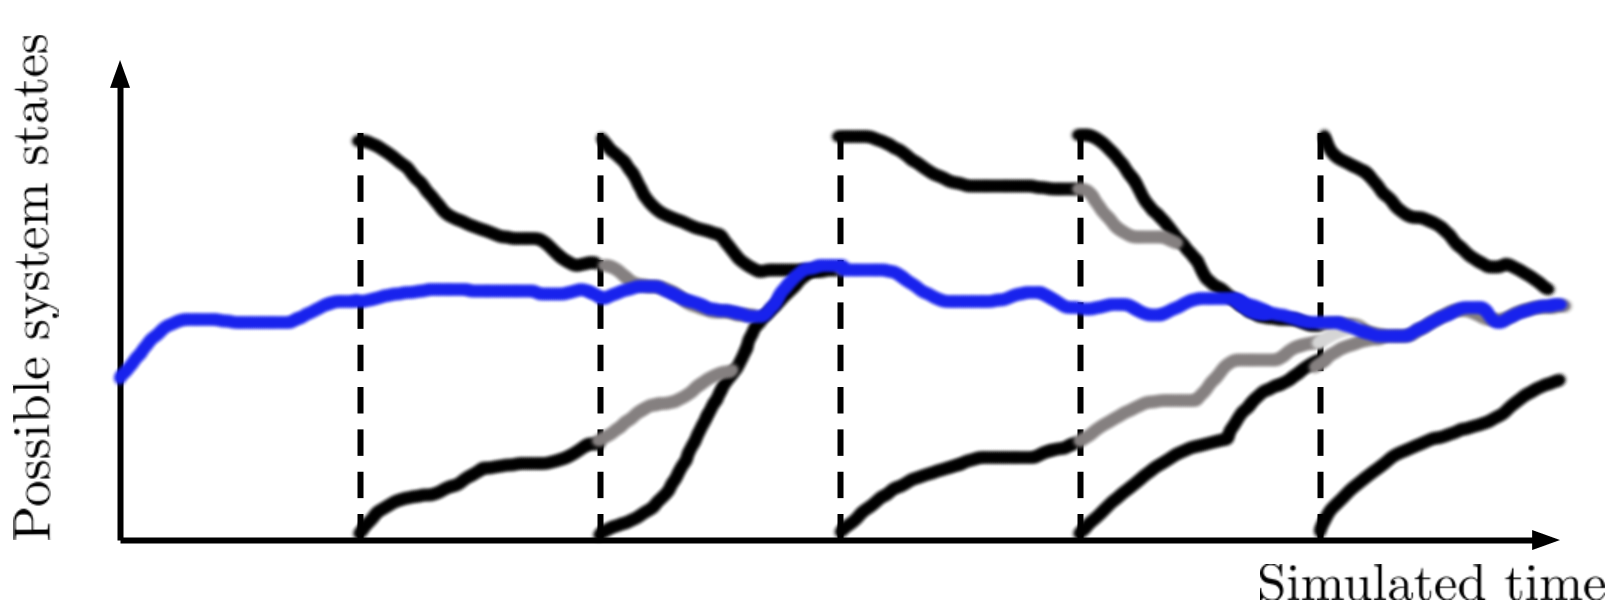
\includegraphics [width=\textwidth]{step3} 
	   
	   Step 4
\end{frame}

\begin{frame}{Variantes }

Variantes de l'algorithme :
 \begin{itemize}
 \item Choix de l'intervalle à traiter par un processeur :
 \begin{itemize}
 \item Plus petit indice possible
 \item Privilégier l'intervalle le plus en "retard"/ le plus loin de coupler
 \item Chaque processeur calcul la même zone d'intervalles
 \end{itemize}
 \item Choix du nombre d'intervalles
 \end{itemize}
 \vspace{1cm}
 Optimisations
   \begin{itemize}
 \item Ne pas calculer le dernier intervalle tant que l'avant dernier n'a pas couplé
 \item Ne pas recalculer un intervalle couplé, même si ses bornes de départs sont meilleures
  \end{itemize}
\end{frame}


\begin{frame}{Algorithme à une borne (One bound) }

On comparera l'algorithme avec une seule ou deux bornes.
\vspace{1cm}

Utiliser une seule borne pour la simulation temps parallèle :
\begin{itemize}
\item Divise le temps de calcul d'un intervalle par deux
\item Plus de couplage, mais monotonie augmente la chance que les trajectoires se croisent
\end{itemize}
\end{frame}


\begin{frame}{Implémentation en distribué }
\begin{block}{Spécificités technique}
Implémentation de l'algorithme sur des raspberry-pi 3 b connectés en réseau local en ethernet
\end{block}

\begin{block}{Protocole réseau}
Utilisation des sockets en C, avec TCP/IP

$\rightarrow$  Temps réseau coûte cher à cause de la taille des messages et de TCP
\end{block}

    Résultats sur $7$ esclaves et $1$ maître.
	   
\end{frame}


\begin{frame}{Experiences sur un tandem de files d'attentes}
  \centering
    \includegraphics [width=\textwidth]{tandem} 
    
    Les paramètres $a_i$, $d_i$ et $s_i$ et le nombre de files sont fixés de façon à avoir un grand temps de coupalge.
    

  \end{frame}
  
  \begin{frame}{Résultats - Temps de couplage $>$ temps de simulation}
  \centering
    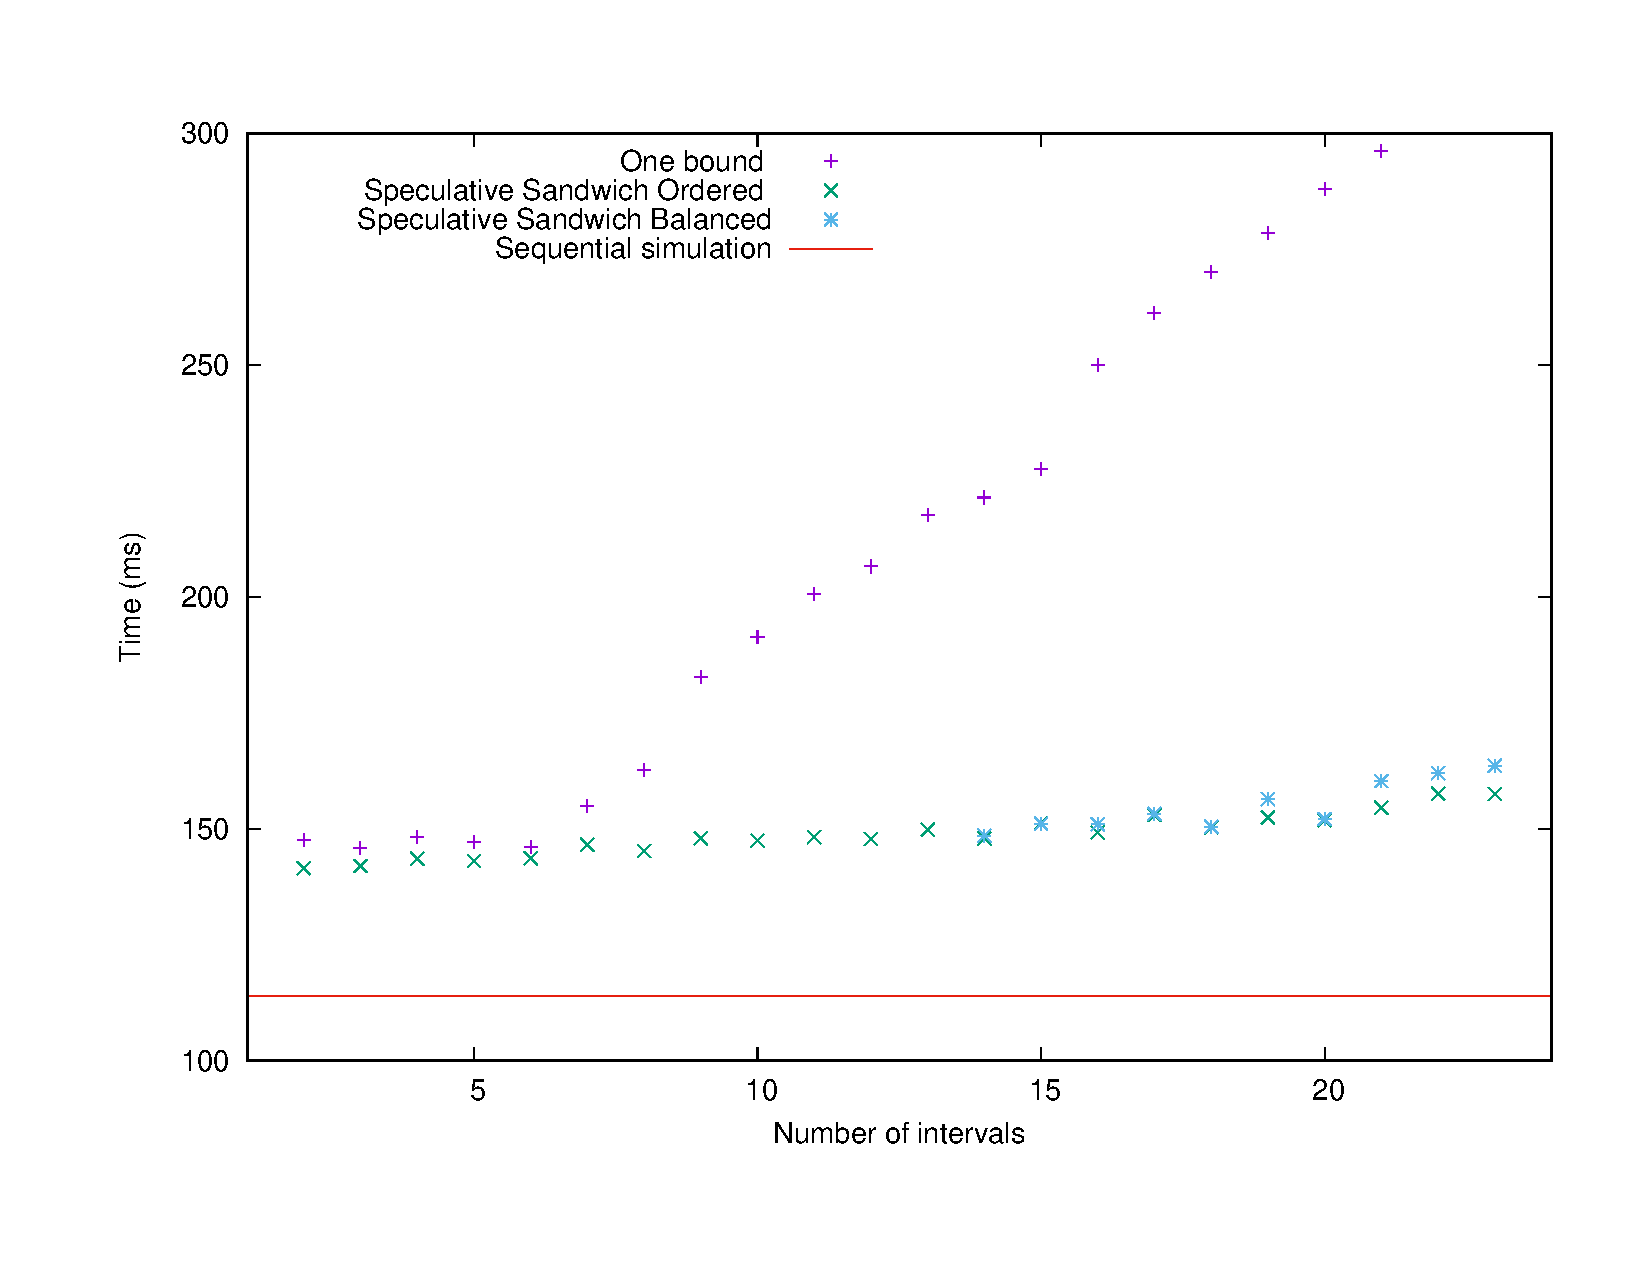
\includegraphics [width=0.9\textwidth]{time_short} 
    

  \end{frame}


  \begin{frame}{Résultats - Temps de couplage $\simeq$ taille d'un intervalle}
  \centering
    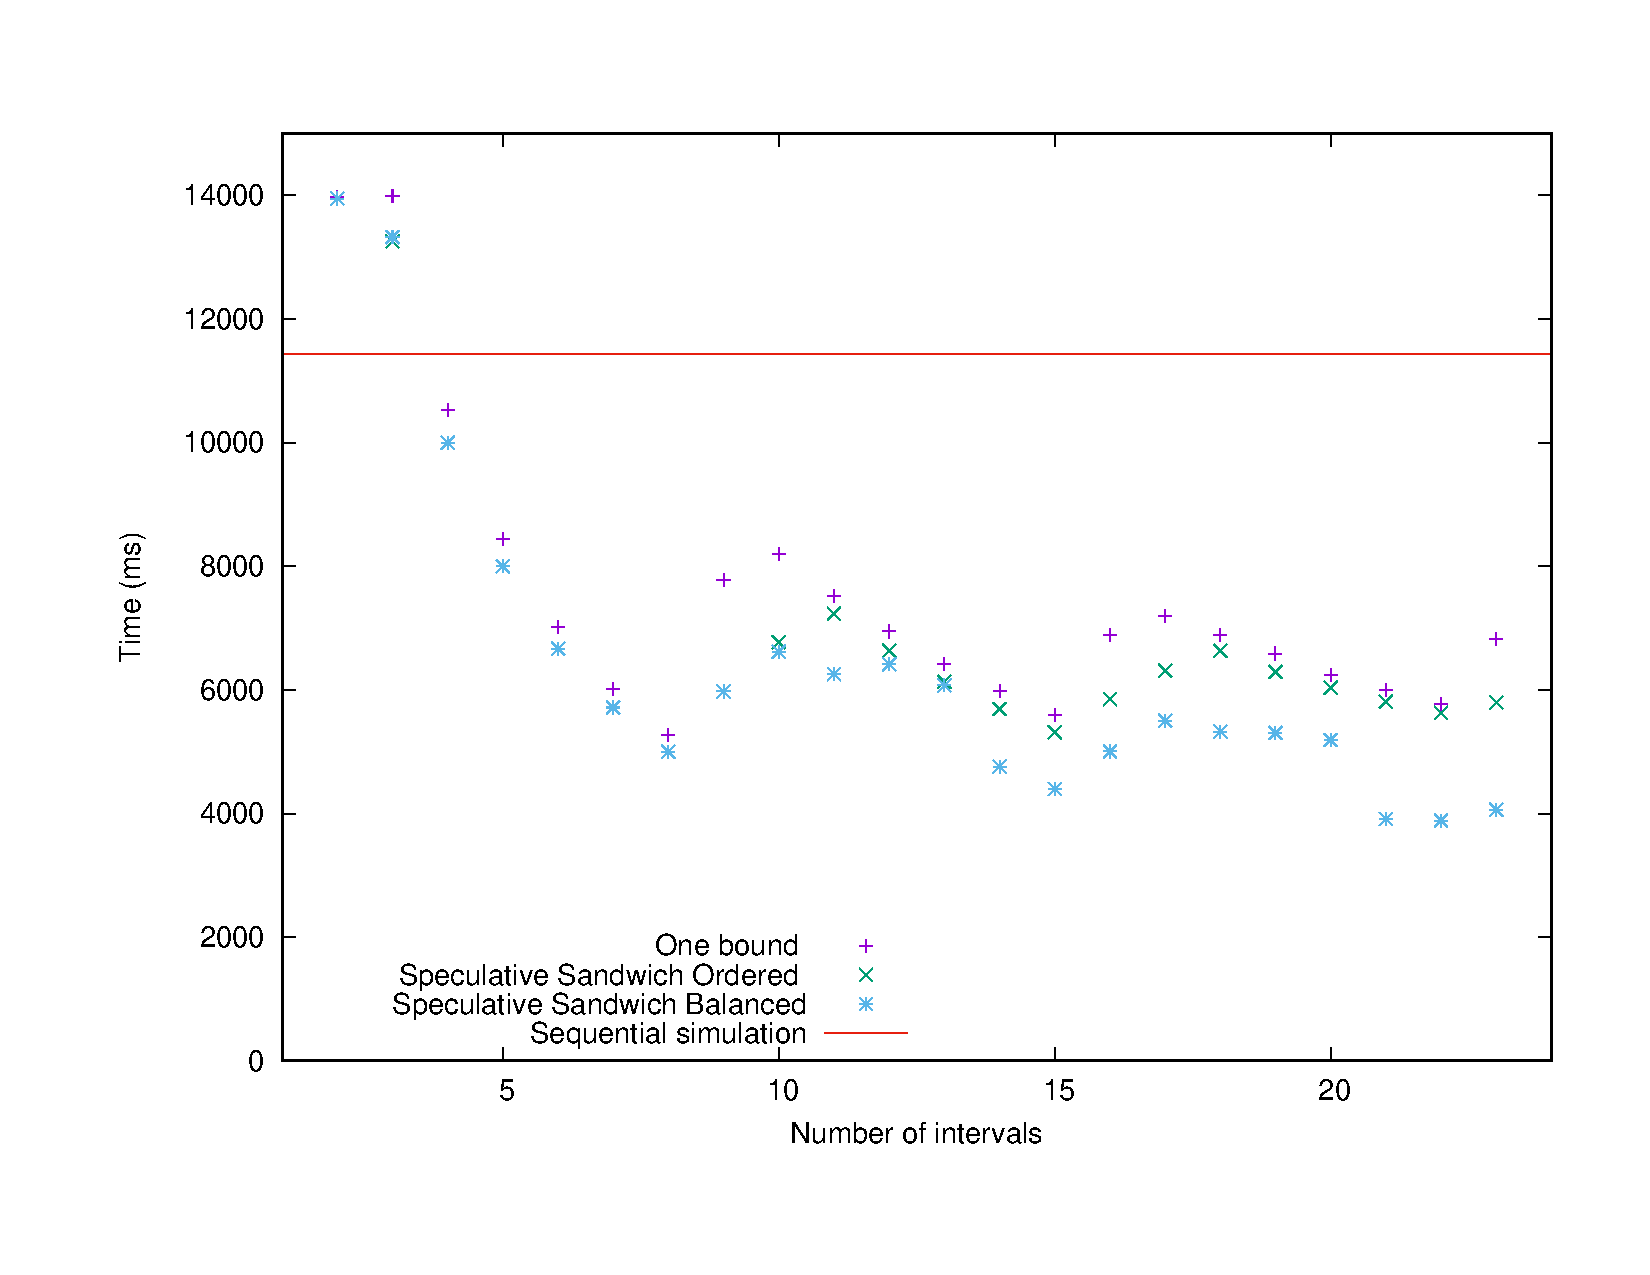
\includegraphics [width=0.9\textwidth]{time_long} 
    

  \end{frame}
  
    \begin{frame}{Impact du nombre de processeurs}
  \centering
    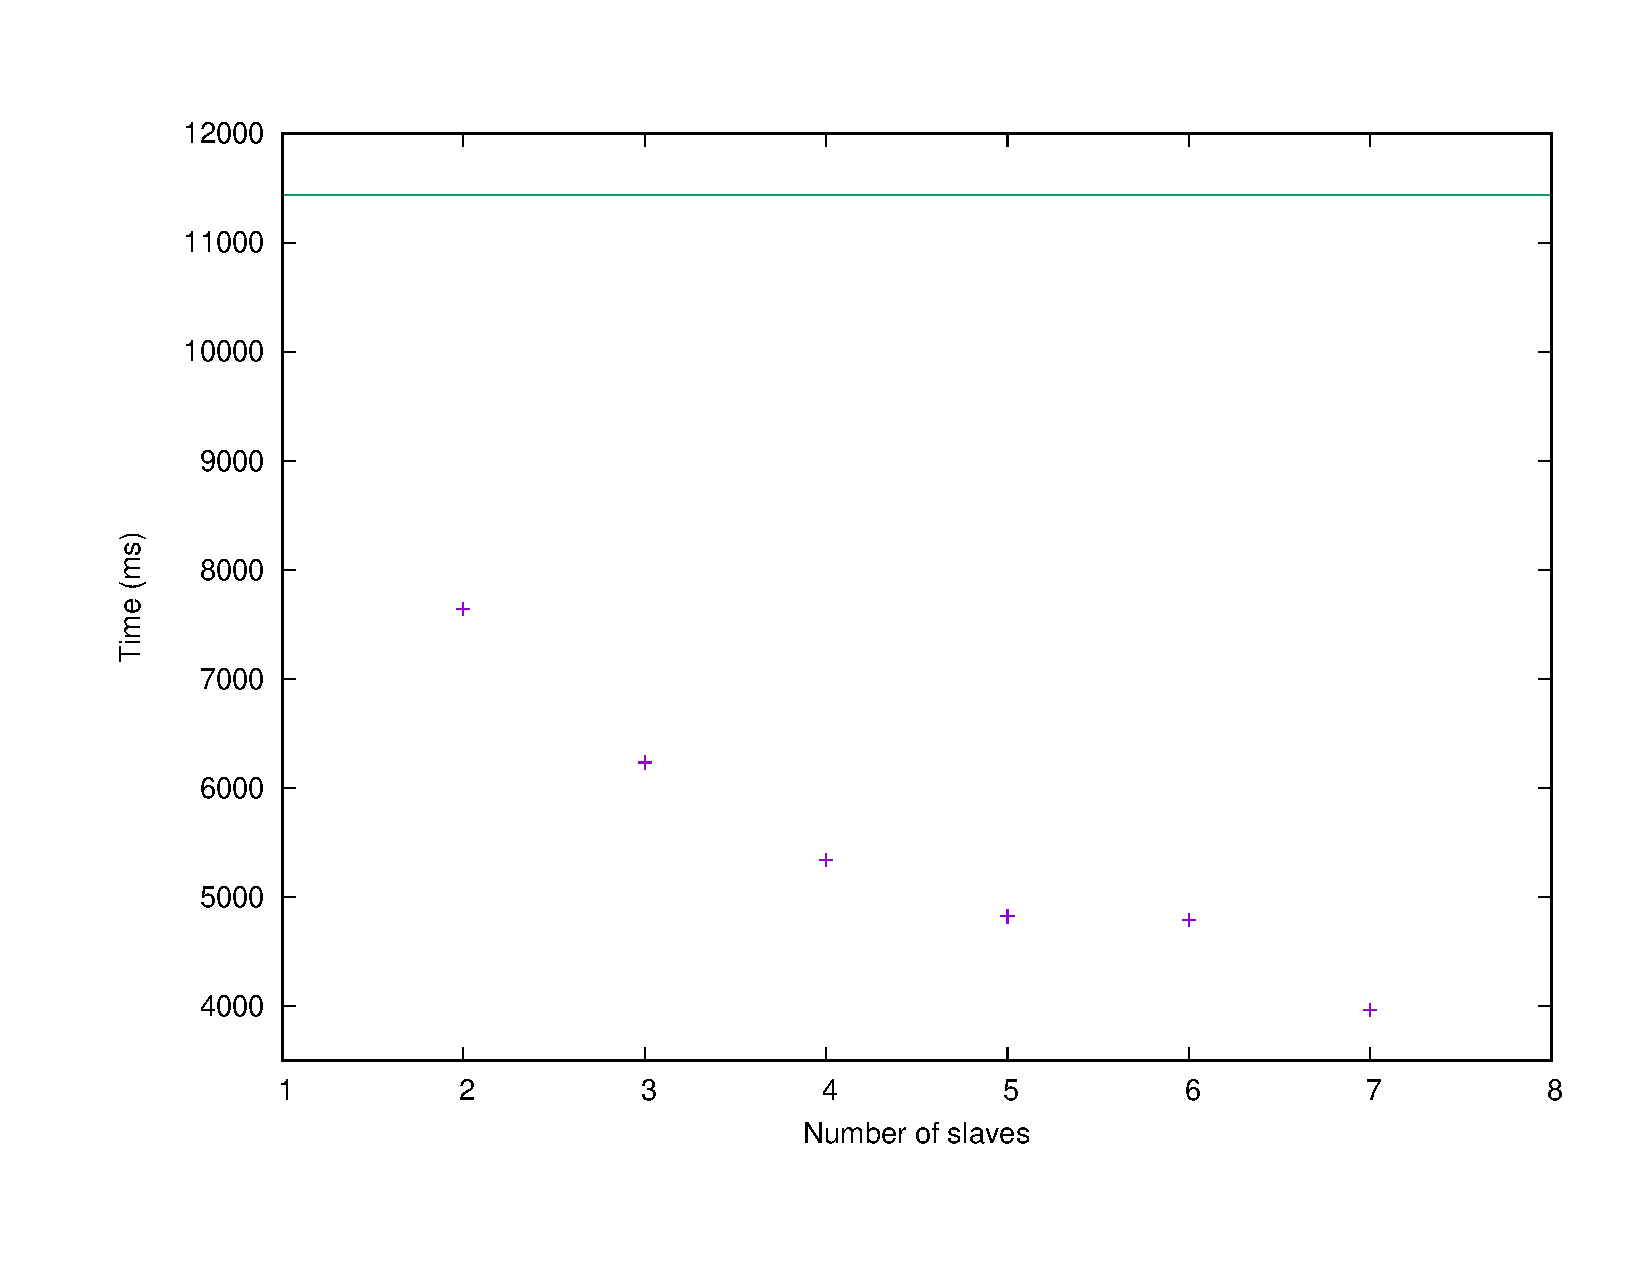
\includegraphics [width=0.9\textwidth]{numberofservers} 
    

  \end{frame}


  \begin{frame}{Variante d'implémentation - OpenMP}
  \centering
  Utilisation d'une machine multiprocesseur et d'une implémentation OpenMP:
  \begin{itemize}
\item On supprime les temps de communication réseau.    
\item Besoin de gérer les locks : coûteux.
   \end{itemize}
\vspace{1cm}
Accélération de presque \textbf{le nombre de processeur} quand les deux bornes couplent très vite !
  \end{frame}

  \begin{frame}{Conclusion}


Algorithme plus performant que le séquentiel.
\vspace{1cm}

Programmé sur OpenMP et sur plusieurs machines.
\vspace{1cm}

Comment choisir les intervalles à calculer, estimer le nombre d'intervalles à choisir?
\end {frame}

  \begin{frame}{Conclusion}

\centering
Merci de votre attention.
\end {frame}

\end{document}
